\color{blue}


数字媒体使用的兴起以及与互联网几乎不间断连接的能力引发了许多关于互联网使用如何影响认知能力的担忧。 
互联网使用如何影响青少年的认知发展?家长和政策制定者越来越多地表达他们对互联网使用对发展中的青少年一代的影响的担忧(George&Odgers,2015)。

从两个方面定义 “人机强交互” :“人机交互”、 “强交互”(高强度、高频率、长期重复)

\section{人机交互}
\textbf{起源}

人机交互研究最初是以机器为中心, 心理学家训练选拔员工以适应机器。后来二战期间机器复杂到难以使人适应, 研究重心才转移到以人为中心,(.....)[\cite{} 人机交互研究综述,2017]

{\textbf 发展}

人机交互有多种形式, 从最初的发展到现在经历了三代的更替。更替的过程彰显了从“硬交互”到“软交互”的过程。 第一个交互时代是鼠标加键盘的时代……第二个交互时代是触摸交互时代, 使人们的双手从键盘和鼠标中解放出来,人与机器的交互变得更 加直接和简单 ……第三个交互时代是感官交互时代,在这个时代,人机交互已经不需要直接的接触,身体控制、感官交互占据主流……[\cite{}, 新媒体语境下的人机交互叙事初探,2018]。人类与机器间的共生合成体可以说是正在形成……而这种合成体威胁了我们这种感觉的稳定性。 人类创造了电脑,接着电脑又创造了新型的人,这也许正在悄然发生。[\cite{}马克·波斯特.信息方式[M].范静哗.译,北京:商务印书馆,2000:11 ]


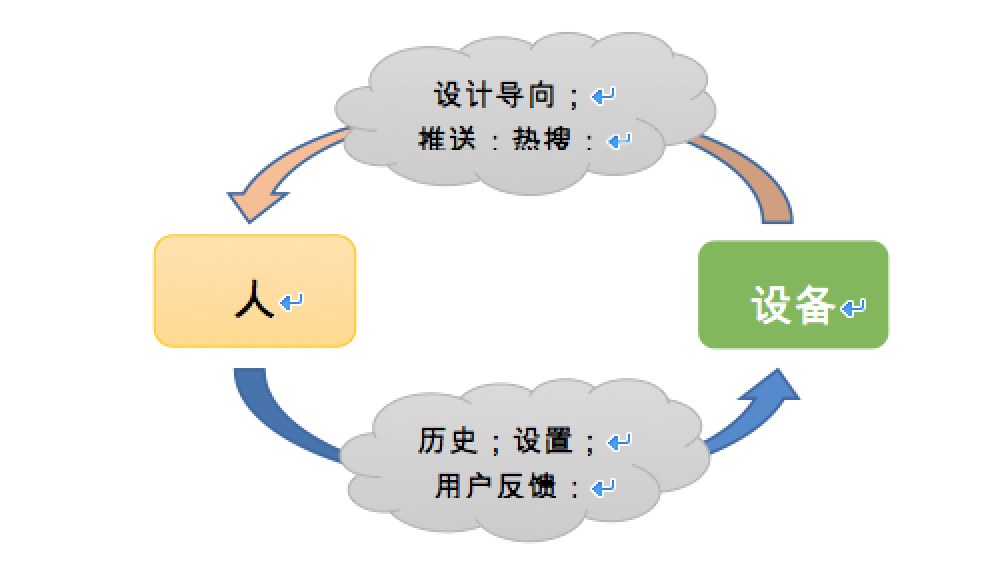
\includegraphics[scale=0.6]{人机交互}


\section{“强”交互}


随着互联网,特别是移动互联以及人工智能技术的发展,信息技术对社会、经济、教育等基础领域持续地进行塑造与变革。人类生活的各个方面都得益于信息技术渗透从而取得巨大的发展。信息技术给社会生活带来的重要影响之一是人们与电子设备会长时间持续的交互。例如,类似Facebook, QQ, 微信等在线社交平台的兴起,人们每天会长时间的使用这些软件平台。以微信为例,人们平均在微信上花费的事件达到了2-3小时。Facebook这些社交软件的日活跃用户也达到了2亿。在青少年中盛行的社交软件是腾讯的QQ。另一个例子就是电子游戏。腾讯的主要收入就是来自于它的游戏产业。这些游戏主要玩家就是青少年。机器和设备对于“人的影响”日益明显,甚至正在 “创造新型的人”,这和其本身的存在形式的演变不无关系。

由于移动设备带来的便利性使得人们产生信息和内容的方式发生了根本性的变化,导致了信息呈现爆炸式的增长。%移动互联时代下的信息爆炸式增长可以分别从主动推送和被动接收两个方面来说明。
一方面,信息主动推送的来源丰富:
\begin{enumerate}
\item 原来的论坛或者博客,乃至门户网站,其信息都是定时更新。而有了微博、微信则变成了随时、随地都可以发送信息和图片等。信息发送本身不再受空间、时间的限制了;

\item 再次,由于有了关注和交互,任何一个内容的产生我们可以有大量的转发和评论,而评论本身即是对信息内容的再次加工,又变成了一条信息的信息,大V或网红发送信息或热点事件本身,往往会产生大量指数级增长的评论信息,这本身也是信息爆炸的一个点;

\item 此外,还有就是随着物联网和传感技术的发展,我们采集信息或数据的方式发生了巨大的变化,比如对于温度,水压检测,我们可以通过传感器实时的采集数据,而不是类似传统方式定时人工记录,这些自动化采集技术的发展本身也极大增加了信息扩张的速度。
\end{enumerate}

另一方面,大量信息通过基于被动推送的方式获取,如高频率使用的微博,微信,知乎等平台。而这些平台基本都是通过关注他人或关注话题获取到实时的信息推送,这些信息推送往往是一种被动的信息接收过程。或者说这些渠道占据了我们一天绝大部分的信息来源,导致对如新浪这一类新闻门户网站访问的兴趣、热情、频率日渐下降。在基于被动推送的海量信息获取方式下,儿童、青少年由于其认知能力发展不成熟,容易产生互联网过度使用甚至成瘾,会进一步造成认知障碍。被动推送以获取信息的方式具有的主要特点包括,
\begin{enumerate}
\item 我们能接收到的信息往往来自我们关注的人。由于对人的关注,导致我们不得不被动接收该人发出的所有其它我们并不感兴趣的内容,%,比如我关注了一个IT专家,但是他可能每天更多发布的是儿子照片或美食图片,而不是我真正关心的内容,
这本身也可能增加信息噪音。
%特别是大V的影响,如果这些人没有产生或推送出某条信息,那么在我们的TimeLine上往往就没有任何信息显示。%虽然当前也有话题关注的功能,但是这个功能往往用的并不多,除非出现特别热门的话题,我可能才会进入到微博的话题关注中。

\item  同样,正是出于对人的关注,而不是对知识点或内容本身的关注,很多高质量的内容往往并不会推送到你的时间线上%,而如果有大V愿意转发你的内容,往往就容易引起一个指数级的引爆传播。
 
\item 出于对人的关注,我们一方面获取的不是最原始核心的知识结构,更多是大V加工后和处理后的信息、而另一方面由于常时间被动接受信息,思维更加容易受到他人影响而丧失独立思考。
\end{enumerate}

这些都是信息爆炸可能导致认知瓶颈和认知障碍的核心原因。

据前所分析,随着信息爆炸式增长,人机高强度、高频度的交互环境已经成为人类生活不可或缺的部分。因此,在现有的“人机交互”的基础上,我们尝试提出“人机强交互”的概念,并进一步探究“设备”对人的影响。
我们将这些人们与电子设备或平台交互非常频繁的环境称为人机强交互环境,其特征包括人与智能计算机(包
括计算机、智能终端、电子设备、虚拟现实场景)在高冲击力、多群体、高频度、高密度、富信息、碎片化的场景下的交互。人机强交互包括以下三个特征:
\begin{enumerate}
\item 刺激强度

	设备对使用者的刺激是高冲击力的、多群体的、高频度的、高密度对、富信息的、碎片化的。
	
\item 软件的“沉浸式设计”

	各类产品的“沉浸式设计”是加强人机交互强度的直接因素,这是一个涉及到心理、设计、游戏等领域的概念。


软硬件设计本身就具有明显的导向性,例如抖音等小视频软件的诱导性,包括吸引用户发布视频和游客“沉浸”于浏览视频,微博等公众社交媒体“热搜”等设置有明显的舆论导向甚至价值导向作用;而用户的个人设置,浏览记录等信息使得媒体“更好地”针对性推送内容,使用户与设备的联系进一步加强,大数据背景下的用户反馈又是促使媒体优化设计的重要影响因素,使得“人机交互”成为一个持续的双向强化过程,并在这个过程中打造出一个针对用户个体的适宜、偏好和易沉浸的“强交互环境”。


\item 相互反馈


人机“强交互”语境下,存在一个使用者与机器相互反馈,影响双方行为的过程,并逐渐形成相对稳定的交互关系,使得用户个人与其设备构筑成为一个共生的“强交互环境”。
\end{enumerate}

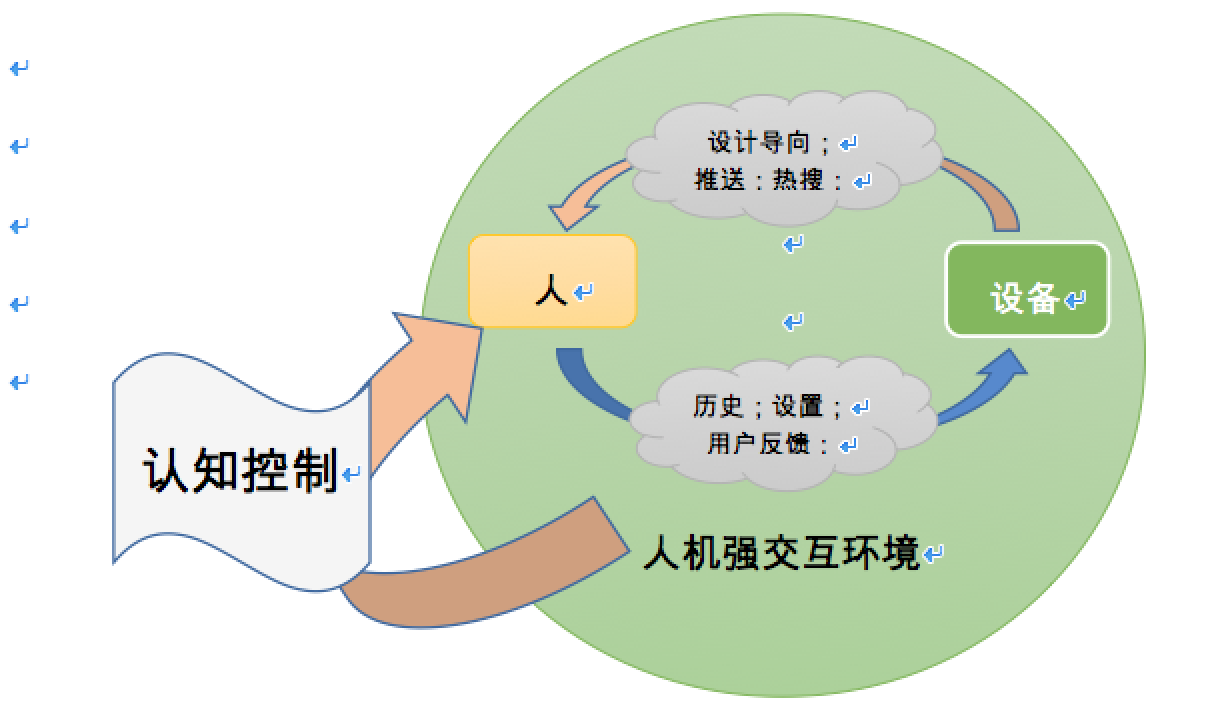
\includegraphics[scale=0.5]{人机强交互-认知控制}



因此,要研究当前时代环境对青少年的影响关系,人机强交互环境的是一个重要的突破点。

\section{儿童青少年的互联网使用现状}

要了解互联网使用如何影响青少年的认知发展,首先需要描述青少年如何使用互联网。

美国:在2014年底和
2015年初,皮尤研究中心调查了互联网使用1060名13至17岁的美国青少年(Lenhart,2015)。在这些样本
中,92%的人报告每天使用互联网,其中24%的样本几乎不停地上网。在这次调查中,拥有移动设备的青少
年比没有青少年的青少年更有可能频繁访问互联网。移动设备,94%的青少年从移动设备访问互联网至少可
以上网,而68%的青少年没有通过移动设备访问互联网(Lenhart,2015)。最近的全国互联网使用调查表
明,青少年经常使用互联网,但不限于从固定设备访问互联网。

青少年报告参与各种在线活动,但从社交网站到多人视频游戏的互联网使用的许多方面都涉及与同龄人交
流。在一项针对128名美国13至14岁儿童的访谈中,85%的人报告使用信息技术进行交流(Fitton,
Ahmedani,Harold,&Shifflet,2013);一项针对6个欧洲国家的10,930名青少年的研究发现,大约70%的
14至18岁的青少年每天都使用社交网站(Tsitsika等,2014)。青少年使用社交网站的主要原因是为了与离
线知名的个人建立联系(Reich,Subrahmanyam,&Espi-noza,2012)。

一个重要但很少被提及的考虑因素是大多数互联网使用的多任务处理性质。 2015年常识普查报告声称,数字媒体的使用(包括互联网使用)可以与其他活动同时发生,如锻炼,家务或通勤(Common Sense Media,2015)。因此,使用互联网并不一定取代其他活动的参与。更复杂的是,在线社交可以与离线社交同时进行,因为社交媒体使用也是可以在同一离线环境中出现的那些朋友之间共享的活动(类似于视频游戏)。
最后,2014 - 2015年皮尤研究中心青少年关系调查表明,互联网使用可能实际上是补充,而不是取代面对面沟通的时间,因为与他们最亲密的朋友一起在学校(83%)或在家里(58%)的青少年比那些与他们最亲密的朋友在网上花时间的青少年(55%)多(Lenhart,Smith,Anderson,Duggan,&Perrin,2015)。虽然许多玩电子游戏的青少年也与其他在线“游戏玩家”一起玩游戏(75%),但更多的人倾向于和朋友一起玩视频游戏(89%)(Lenhart等,2015)。

欧洲

\subsection{国内数据}

温州

台湾


\subsection{国外数据}


\subsection{影响}

\begin{enumerate}
\item 设备使用频率和时长的增加

	在“人机强交互环境”中,人们对设备的使用频率在增加(时不时看手机),使用的持续时间变长(一看就是好几十分钟甚至几个小时),使用时的“浸入程度”也在加深(走路都要看,掉下水道里去!)。
		这中现象对人们的生活带来……的直接影响,也在悄然改变我们的思维和认知习惯……
\item 当我们每天翻看手机上的社交平台,阅读那些看似有趣和有深度的文章时,我们正在渐渐丧失深度阅读和深度思考的能力。


\end{enumerate}


互联网鼓励我们蜻蜓点水般地从多种信息来源中广泛采集碎片化的信息,其伦理规范就是工业主义,这是一套速度至上、效率至上的伦理,也是一套产量最优化、消费最优化的伦理。互联网正在按照自己的面目改造我们,我们变得对浏览和略读越来越得心应手,但是我们正在丧失的却是专注能力、沉思能力和反省能力。


\section{小结}

c.f. Possible Effects of Internet Use on Cognitive Development in Adolescence\cite{Mills2016})

正如最近的观点所述(George&Odgers,2015; Mills,2014),仍然缺乏实验研究来检验互联网在认知发展中的使用影响。目前的评论侧重于少数几项研究,这些研究研究了互联网使用对青少年和新兴成人认知过程的可能影响,包括社会认知过程。

互联网使用如何影响认知的问题并不简单,不能通过一个甚至一系列实验来回答。互联网使用可被视为环境
暴露变量,类似于音乐训练或营养不良。然而,与音乐训练或营养不良不同,互联网使用是近年来几乎所有
工业化国家都面临的环境因素。这使得几乎不可能进行实验比较有和没有接触互联网的群体。实际上,关于
互联网使用的一个主要问题不仅仅是如何使用互联网影响记忆或社会理解等认知过程,而是如何不断访问互
联网可能会影响这些认知过程。
考虑到二十年代认知过程的持续发展,研究互联网使用对青少年认知的影响是有必要的(Luna,Marek,
Larsen,Tervo-Clemmens,&Chahal,2015)。 这些认知过程包括但不限于\textcolor{red}{工作记忆能
力,注意力控制和社会认知}。 \textcolor{red}{关于互联网如何影响青少年认知发展的具体问题包括,如何近
乎持续地获取信息可能会破坏记忆能力或努力思考的利用(Näsi&Koivusilta,2012),或在几个在线/离线
活动之间的多任务能力如何缩短注意力}。 虽然这些关于认知能力改变的担忧通常都在“互联网使用可能重
新改变发育的大脑中的神经连接”的观念中,但目前的观点主要集中在认知过程而不是相关神经或神经发育
上。

 本综述将最新的互联网使用经验证据与相关实验研究相结合,探讨在线行为和在线环境结构如何影响儿童青
 少年的认知发展。 根据所审查的证据讨论了备受关注的问题。


